%!TEX root = ../../Heun_Dale_Haney_A_dynamic_approach_to_input_output_modeling.tex
%%%%%%%%%%%%%%%%%%%%% chapter.tex %%%%%%%%%%%%%%%%%%%%%%%%%%%%%%%%%
%
% sample chapter
%
% Use this file as a template for your own input.
%
%%%%%%%%%%%%%%%%%%%%%%%% Springer-Verlag %%%%%%%%%%%%%%%%%%%%%%%%%%
%\motto{Use the template \emph{chapter.tex} to style the various elements of your chapter content.}


%%%%%%%%%%%%%%%%%%%%%%%%%%%%%%%%%%%%%%%%%
%%%%%%%%%% Direct Energy Flows %%%%%%%%%%
%%%%%%%%%%%%%%%%%%%%%%%%%%%%%%%%%%%%%%%%%
\chapter{Direct energy flows}
% Always give a unique label
\label{chap:direct_energy} 
% use \chaptermark{} to alter or adjust the chapter heading in the running head
\chaptermark{energy}
%%%%%%%%%%%%%%%%%%%%%%%%%%%%%%%%%%%%%%%%%
%%%%%%%%%%%%%%%%%%%%%%%%%%%%%%%%%%%%%%%%%
%%%%%%%%%%%%%%%%%%%%%%%%%%%%%%%%%%%%%%%%%


\abstract*{[NEED TO ADD ABSTRACT HERE]}

%% \abstract{Each chapter should be preceded by an abstract (10--15 lines long) that summarizes the content. The abstract will appear \textit{online} at \url{www.SpringerLink.com} and be available with unrestricted access. This allows unregistered users to read the abstract as a teaser for the complete chapter. As a general rule the abstracts will not appear in the printed version of your book unless it is the style of your particular book or that of the series to which your book belongs.\newline\indent
%% Please use the 'starred' version of the new Springer \texttt{abstract} command for typesetting the text of the online abstracts (cf. source file of this chapter template \texttt{abstract}) and include them with the source files of your manuscript. Use the plain \texttt{abstract} command if the abstract is also to appear in the printed version of the book.}

%% Use the template \emph{chapter.tex} together with the Springer document class SVMono (monograph-type books) or SVMult (edited books) to style the various elements of your chapter content in the Springer layout.


%%%%%%%%%% Energy: Methodology %%%%%%%%%%
\section{Methodology}
\label{sec:energy_methodology}
%%%%%%%%%%

In Chapter \ref{chap:intro}, we formulated a model of economies
consisting of producers and consumers who exchange
goods and services and factors of production 
while extracting resources and disposing of wastes. 
In Chapter \ref{chap:materials}, we established the material basis of economies: 
economies are analogous to organisms that process raw resources
for the benefit of producers and consumers while generating unavoidable wastes.
In this chapter, we describe and analyze the direct energy that is associated 
with the material flows.

Figure~\ref{fig:PERKS_energy_content} shows a corresponding 
direct energy flow for each material flow of Figure~\ref{fig:PERKS_materials}.
``Direct'' energy refers to forms of energy accounted by the First Law of Thermodynamics,
including chemical potential energy, 
nuclear potential energy, 
gravitational potential energy,
thermal energy, 
and kinetic energy.
We use the term ``direct'' energy as distinct from ``embodied'' energy, 
which will be discussed in Chapter \ref{chap:embodied_energy}.
Examples of direct energy flows include 
the chemical potential energy of coal inflows to an energy sector, 
the thermal energy of process steam into a textile plant, and
the thermal energy of CO$_2$ automobile exhaust.
In each case, the material (coal, steam, and CO$_2$) 
carries direct energy with it.\footnote{Even radiative thermal energy 
can be considered a material flow (photons) that carries
direct energy (thermal) with it.}


\begin{figure}[h!]
\centering
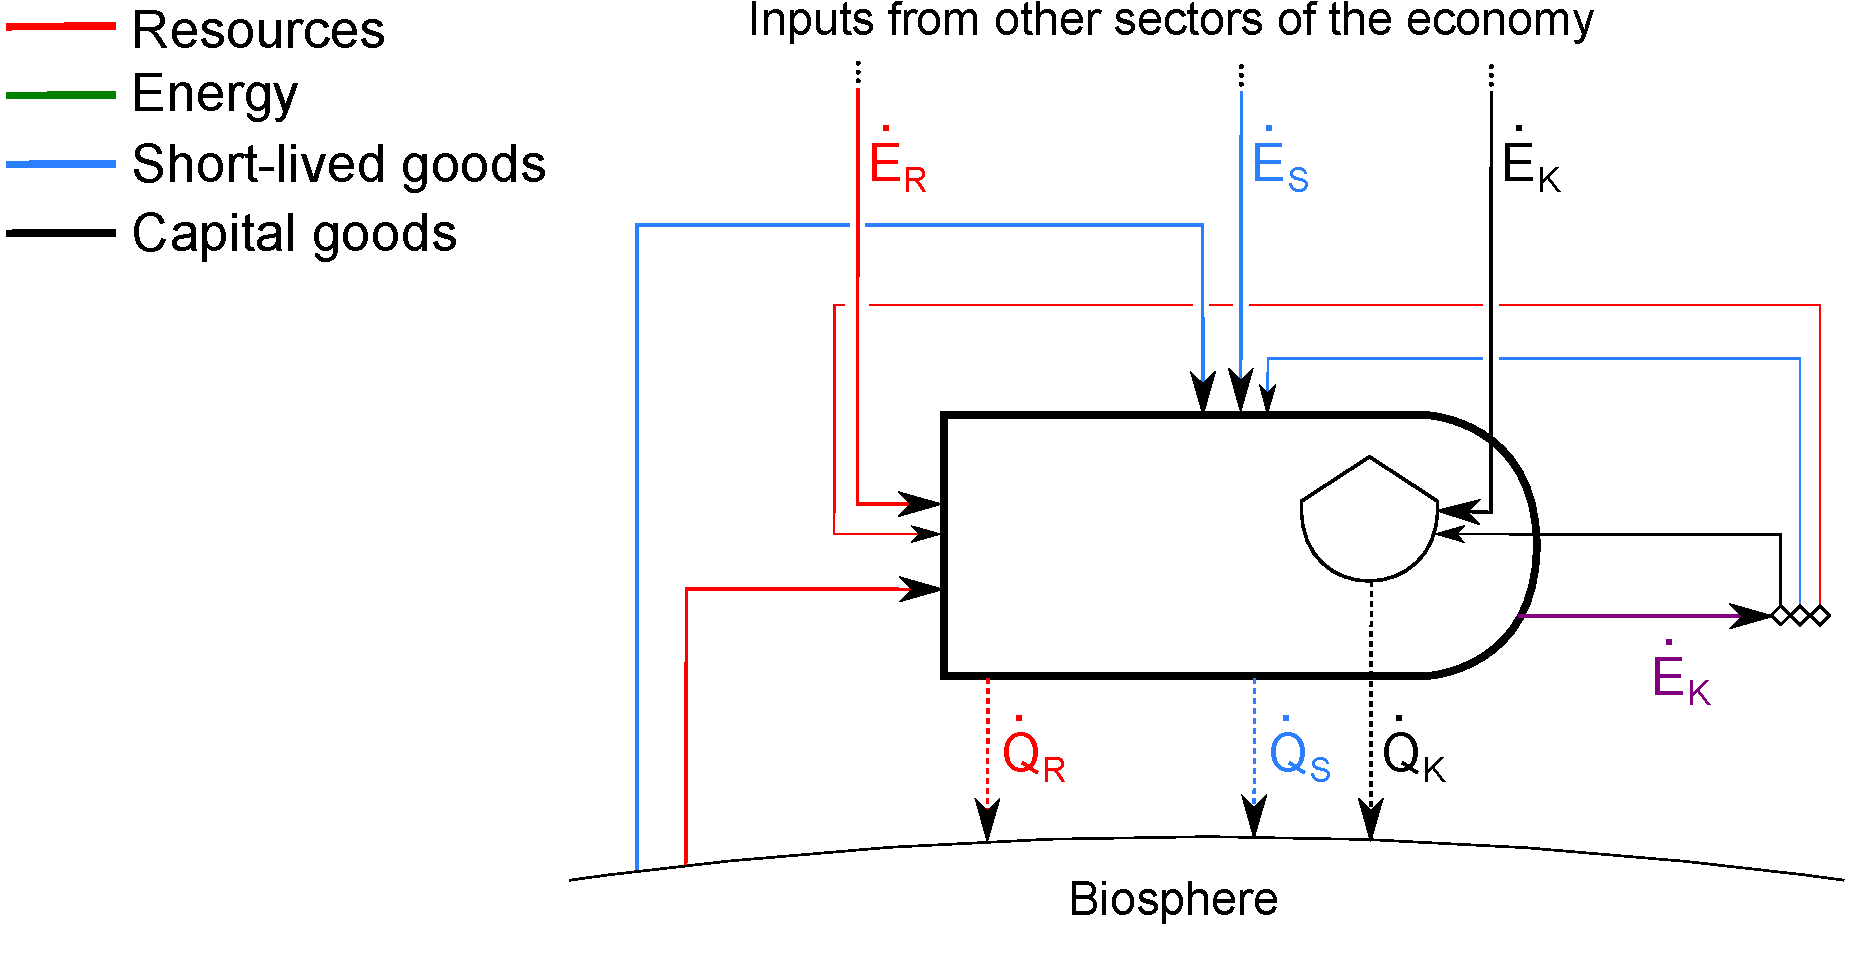
\includegraphics[width=0.8\linewidth]{Part_2/Chapter_Energy/images/PERKS_basic_unit_energy_content.pdf}
\caption{Energy content ($\dot{E}$) of material flows 
($\dot{R}$, $\dot{S}$, and $\dot{K}$) 
from Figure~\ref{fig:PERKS_materials}. 
**** Mik: This figure should not have the green lines. 
The point of this figure is that the $\dot{R}$, $\dot{S}$, and $\dot{K}$ lines 
each have energy associated with them. 
We'll aggregate those lines in the next figure, 
which includes \emph{only} green lines. 
Also, the subscripts should have dots on them: 
$\dot{R}$, $\dot{S}$, etc. 
Can you add an $\dot{E}_{\dot{P}}$ label to the purple line? 
Should we have a net output line pointing to the right
after the product is split apart?
Can we add $\dot{Q}$ labels to the waste lines?
Finally, would it be possible to put the labels 
in the same color as the lines they're labeling? --Matt ****}
\label{fig:PERKS_energy_content}
\end{figure}

For any boundary (around, say, a machine, a plant,
a sector of the economy, or the entire economy itself), 
the First Law of Thermodynamics says that
the accumulation rate of direct energy within the boundary
is equal to the sum of the signed direct energy flow rates ($\dot{E}$)
across the boundary (where inflows are positive and outflows are negative)
less outflowing energy carried by wastes ($\dot{Q}$): 
energy is conserved.

\begin{equation} \label{eq:First_Law_with_accumulation}
	\frac{\mathrm{d}E}{\mathrm{d}t} = \sum \dot{E} - \sum \dot{Q}
\end{equation}

When there is no accumulation of direct energy within the boundary,
$\left( \frac{\mathrm{d}E}{\mathrm{d}t} = 0 \right)$ the sum of all 
signed direct energy flow rates ($\dot{E}$) 
and waste heats ($\dot{Q}$) will be zero.

\begin{equation} \label{eq:First_Law_no_accumulation}
	0 = \sum \dot{E} - \sum \dot{Q}
\end{equation}

It is important to note that the direct energy associated with some material flows can
be very small or negligible compared to other direct energy flows in the economy.
For example, the direct energy of steel into the automobile sector of the economy 
is almost negligible. (The \emph{embodied} energy of the steel is almost certainly
\emph{not} negligible, as will be discussed in Chapter~\ref{chap:embodied_energy}.)
On the other hand, the direct energy flow rates for fossil fuels (coal, oil, and natural gas)
are typically orders of magnitude larger than any others for a given unit of analysis.

To simplify the direct energy analysis, 
we can aggregate the direct energy flows of Figure~\ref{fig:PERKS_energy_content}
into single arrows when appropriate. 
For example, the direct energy inputs from other sectors of the economy
(labeled as $\dot{E}_{\dot{R}}$, $\dot{E}_{\dot{S}}$, and $\dot{E}_{\dot{K}}$ 
in Figure~\ref{fig:PERKS_energy_content}) can be summed to $\dot{E}$ 
(in Figure~\ref{fig:PERKS_energy}) such that

\begin{equation} \label{eq:direct_energy_aggregation}
	\dot{E}_{\mathrm{Fig. \: \ref{fig:PERKS_energy}}} 
	= \dot{E}_{\dot{R}, \: \mathrm{Fig. \: \ref{fig:PERKS_energy_content}}} 
	+ \dot{E}_{\dot{S}, \: \mathrm{Fig. \: \ref{fig:PERKS_energy_content}}} 
	+ \dot{E}_{\dot{K}, \: \mathrm{Fig. \: \ref{fig:PERKS_energy_content}}}.
\end{equation}

\begin{figure}[h!]
\centering
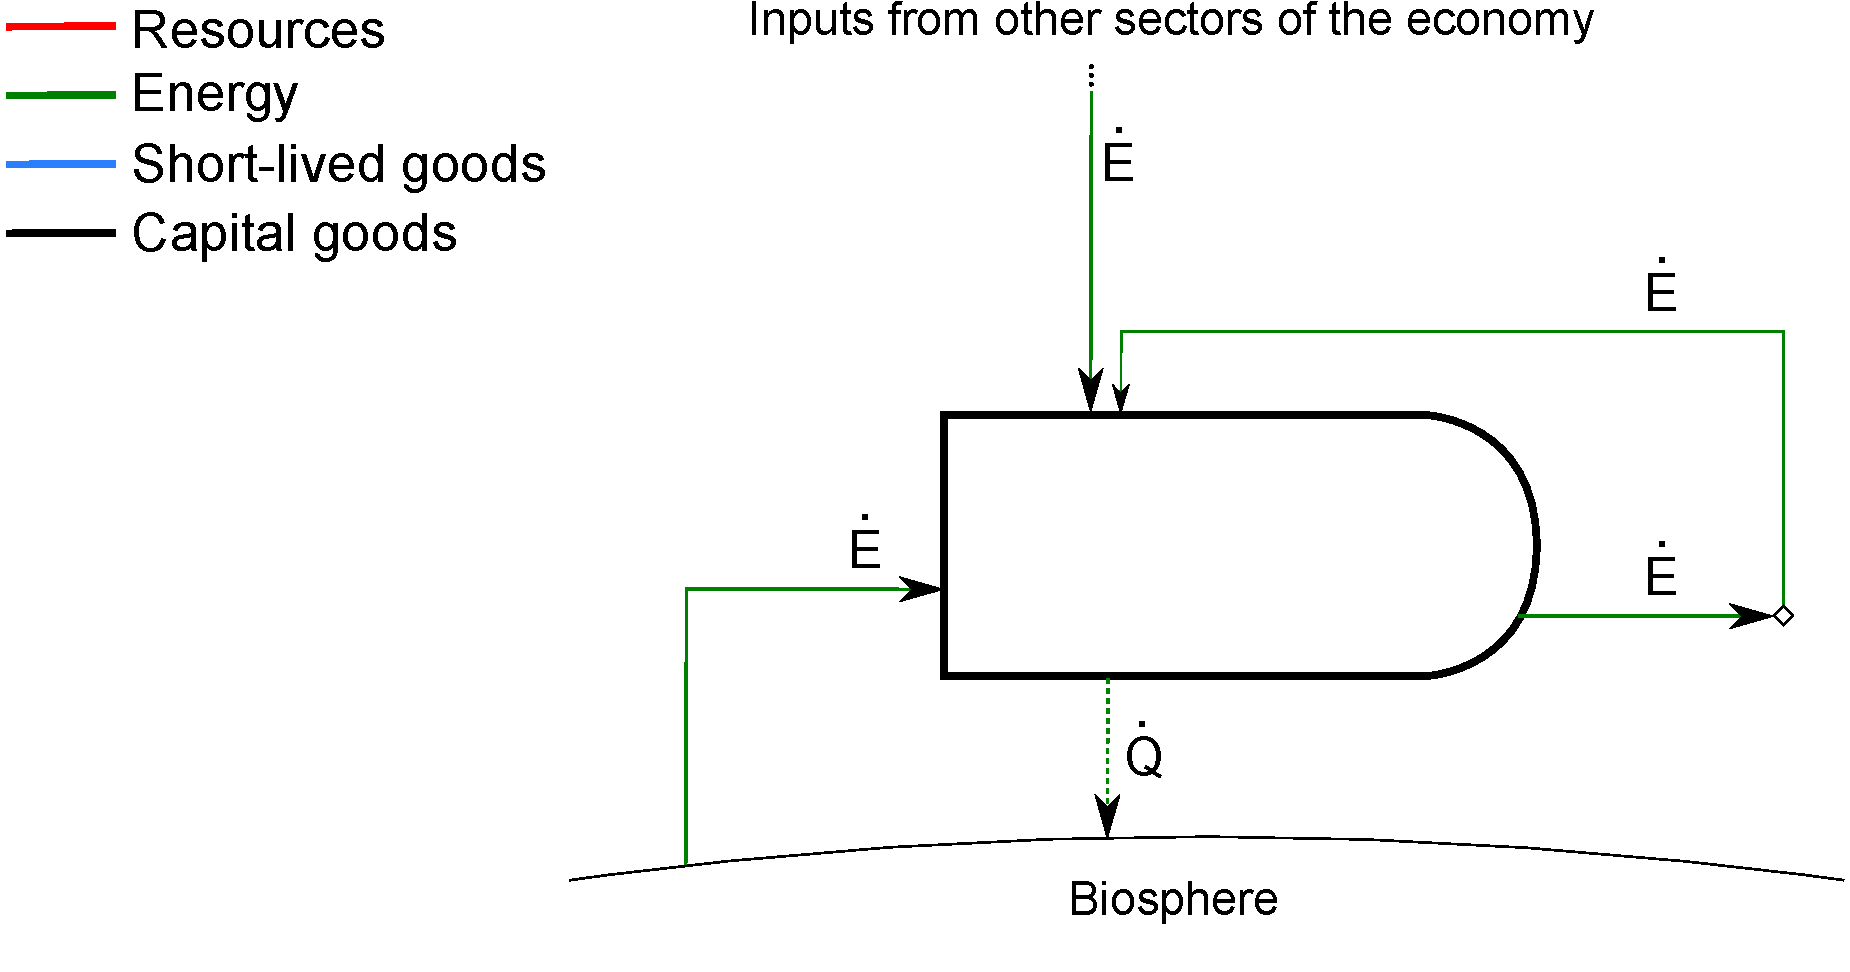
\includegraphics[width=0.8\linewidth]{Part_2/Chapter_Energy/images/PERKS_basic_unit_energy.pdf}
\caption{Aggregated direct energy flow rates around 
the producer of Figure~\ref{fig:PERKS_energy_content}.
**** Mik: remove the subscript ``E'' from the label in this figure. Also, change the 
``E'' to an $\dot{E}$. It's a flow rate. --Matt ****}
\label{fig:PERKS_energy}
\end{figure}


%%%%%%%%%% Energy: Example A %%%%%%%%%%
\section{Example A: single-sector economy}
\label{sec:A_energy}
%%%%%%%%%%

Aggregated direct energy flows are now applied to Example A, 
the single-sector economy shown in Figure~\ref{fig:A_materials}.
By summing the direct energy flows associated with
each material flow of Figure~\ref{fig:A_materials}, we obtain
a simplified picture of direct energy flows in the economy,
as shown in Figure~\ref{fig:A_energy}.\footnote{Single 
subscripts on quantities such as
$E$ can mean one of two things: 
$\dot{E}_{i}$ indicates the outflow of direct energy from sector $i$, 
whereas $E_{i}$ denotes the direct energy content of sector $i$. 
Double subscripts on quantities
(e.g., $\dot{E}_{ij}$) indicate a flow 
from sector $i$ to sector $j$. 
The first index always indicates the sector \emph{from} which a quantity flows, 
and the second index indicates the sector \emph{to} which a quantity flows.}

\begin{figure}[h!]
\centering
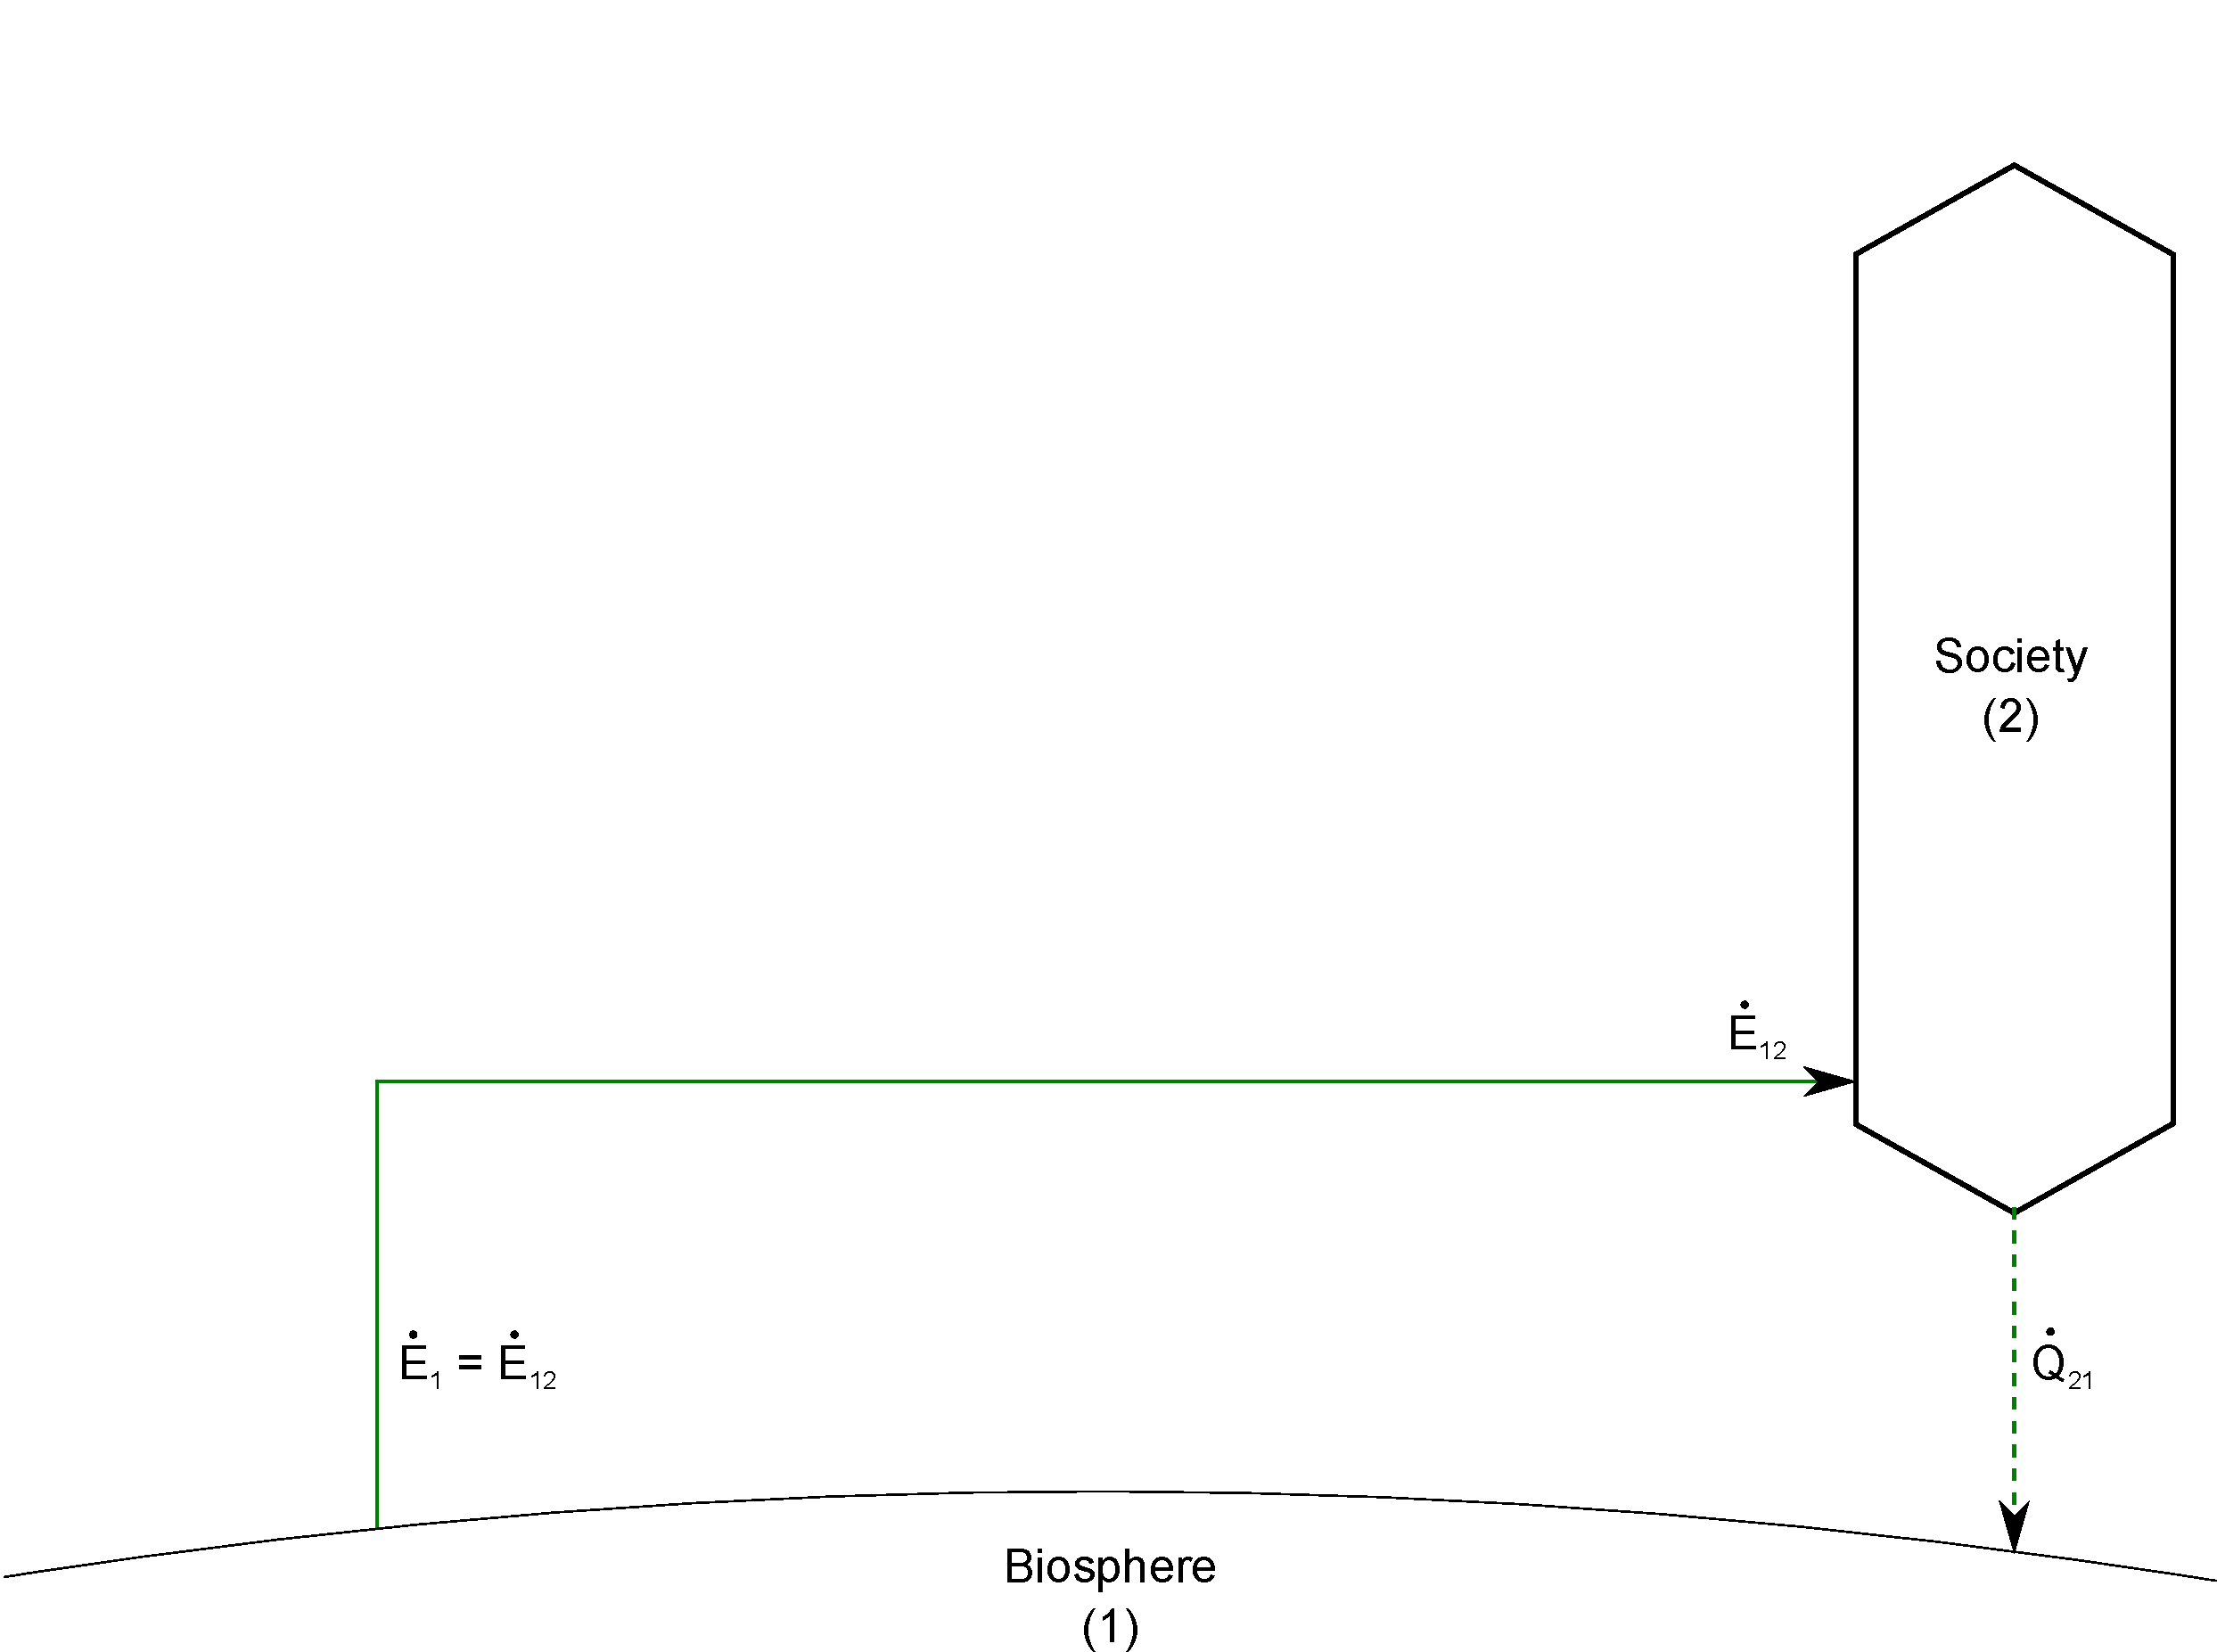
\includegraphics[width=0.8\linewidth]{Part_2/Chapter_Energy/images/1_sector_direct_energy.pdf}
\caption{Direct energy flow rates for Example A, the single-sector economy.}
\label{fig:A_energy}
\end{figure}

We distinguish useful direct energy inputs to a sector of the economy
($\dot{E}_{12}$ in Figure~\ref{fig:A_energy}) from wasteful direct energy flows 
($\dot{Q}_{21}$ in Figure~\ref{fig:A_energy}), 
because $\dot{Q}$ typically denotes thermal energy, 
and most waste energy flows are in the form of thermal
energy, i.e., waste heat. In Figure~\ref{fig:A_energy}, direct energy input to the 
economy ($\dot{E}_{12}$) is shown as being extracted from the biosphere, because
the vast majority of direct energy today is derived from fossil fuel extraction.
Waste heat from the economy ($\dot{Q}_{21}$) is shown as returning 
to the biosphere.

As discussed in Section~\ref{sec:energy_methodology}, 
both direct energy ($\dot{E}$), and waste heat ($\dot{Q}$) 
are accounted by the First Law of Thermodynamics. 
Accounting for possible accumulation of direct energy in the economy, 
the First Law of Thermodynamics for Example~A indicates that

\begin{equation} \label{eq:dE_2/dt_single_sector}
	\frac{\mathrm{d}E_{2}}{\mathrm{d}t} = \dot{E}_{12} - \dot{Q}_{21}.
\end{equation}

Aside from, for example, the U.S. Strategic Petroleum Reserve, 
we are not stockpiling oil and coal at any meaningful rate, 
i.e. we consume fossil fuels at a rate equal to the extraction rate. 
Thus, the world is not accumulating direct energy 
in the economy.\footnote{A counter-example could be made 
for nuclear fuels where ``spent'' fuel represents a large exergetic stockpile. 
However, this reserve is not (presently) economically useful.} 
(The world \emph{is}, however, 
accumulating embodied energy in the economy as we shall see 
in Chapter \ref{chap:embodied_energy}.) 
Thus, the accumulation rate for direct energy 
$\left( \frac{\mathrm{d}E_{2}}{\mathrm{d}t} \right)$ in the above equation 
can be set to zero to obtain

\begin{equation} \label{eq:single_sector_direct_energy_no_accumulation}
	0 = \dot{E}_{12} - \dot{Q}_{21}.
\end{equation}


%%%%%%%%%% Energy: Example B %%%%%%%%%%
\section{Example B: two-sector economy}
\label{sec:B_energy}
%%%%%%%%%%

For Example B, we split the energy sector (3) from 
society (2), assuming that all useful energy for society is 
supplied by the energy sector. Figure~\ref{fig:B_energy} shows aggregated
direct energy flows associated with the material flows of Figure~\ref{fig:B_materials}.

\begin{figure}[h!]
\centering
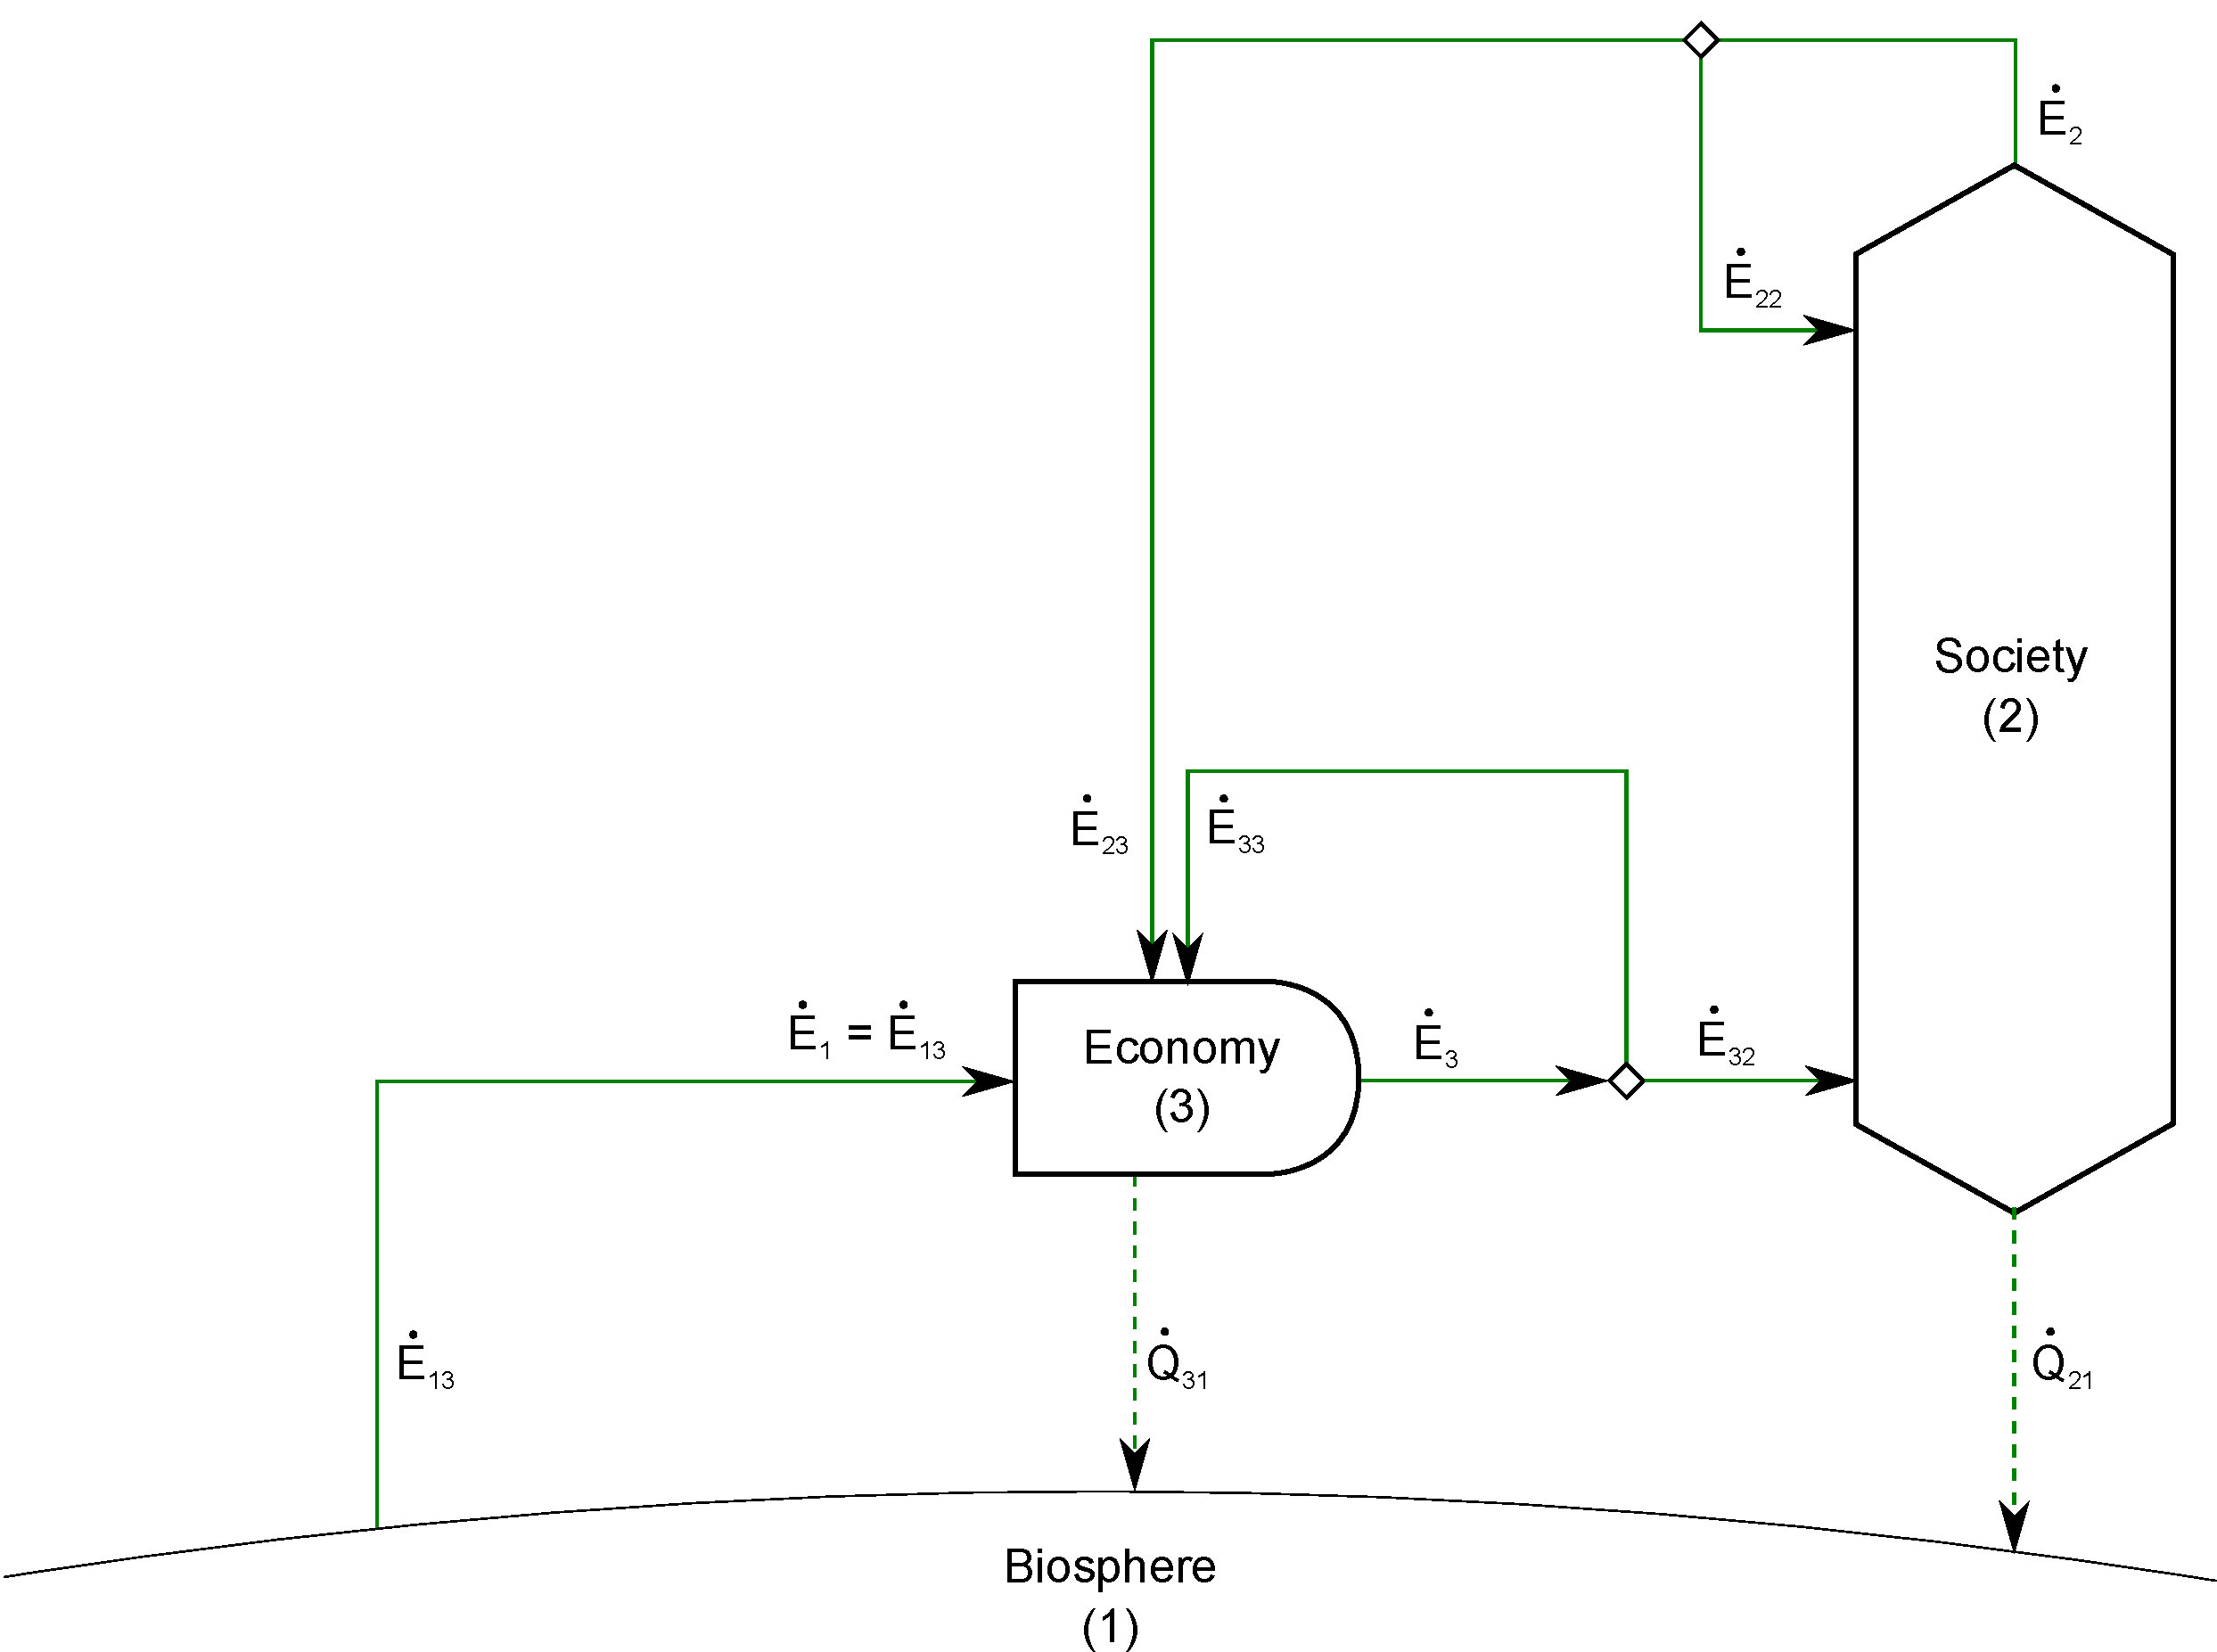
\includegraphics[width=0.8\linewidth]{Part_2/Chapter_Energy/images/2_sector_direct_energy.pdf}
\caption{Direct energy flows for Example B, a two-sector economy.}
\label{fig:B_energy}
\end{figure}

The First Law of Thermodynamics requires that both 
direct energy and waste heat be conserved around each 
sector of the economy (2 and 3) as well as around the biosphere (1).

The First Law around the economic sector (3) 
including the accumulation rate of direct energy in the sector 
$\left(\frac{\mathrm{d}E_{3}}{\mathrm{d}t}\right)$ yields

\begin{equation} \label{eq:CV_E_dot_3}
	\frac{\mathrm{d}E_{3}}{\mathrm{d}t} 
	= \dot{E}_{13} 
	+ \dot{E}_{33} 
	- \dot{E}_{3} 
	- \dot{Q}_{31}.
\end{equation}

\noindent It is notable that sector 3 consumes 
a portion of its own energy output ($\dot{E}_{33}$) 
as it produces its goods and services: it takes energy to make energy.

First Law energy accounting around the biosphere (1) and society (2) gives

\begin{equation} \label{eq:CV_E_dot_1}
	\frac{\mathrm{d}E_{1}}{\mathrm{d}t} 	 
	=  \dot{Q}_{21} 
	+ \dot{Q}_{31} 
	- \dot{E}_{13},
\end{equation}

\noindent and 

\begin{equation} \label{eq:CV_E_dot_2}
	\frac{\mathrm{d}E_{2}}{\mathrm{d}t} 	 
	= \dot{E}_{32} 
	- \dot{Q}_{21}.
\end{equation}

As in Example A, we can set the accumulation of direct energy 
within each sector to zero to obtain

\begin{equation} \label{eq:CV_E_dot_3_SS}
	0 
	= \dot{E}_{13} 
	+ \dot{E}_{33} 
	- \dot{E}_{3} 
	- \dot{Q}_{31},
\end{equation}

\begin{equation} \label{eq:CV_E_dot_1_SS}
	0 
	= \dot{Q}_{21} 
	+ \dot{Q}_{31} 
	- \dot{E}_{13},
\end{equation}

\noindent and 

\begin{equation} \label{eq:CV_E_dot_2_SS}
	0 
	= \dot{E}_{32} 
	- \dot{Q}_{21},
\end{equation}


%%%%%%%%%% Energy: Example C %%%%%%%%%%
\section{Example C: three-sector economy}
\label{sec:C_energy}
%%%%%%%%%%

By adding a goods and services sector (4) to the economy, 
a fuller picture of direct energy flows among sectors is achieved
(Figure \ref{fig:C_energy}). 
In this economy, the purpose of the goods and services sector (4) 
is to produce goods and provide services, 
it provides no direct energy to society. 
The purpose of the energy sector (3) is to make direct energy ($\dot{E}$) 
available to the economy and society in a useful form.

\begin{figure}[h!]
\centering
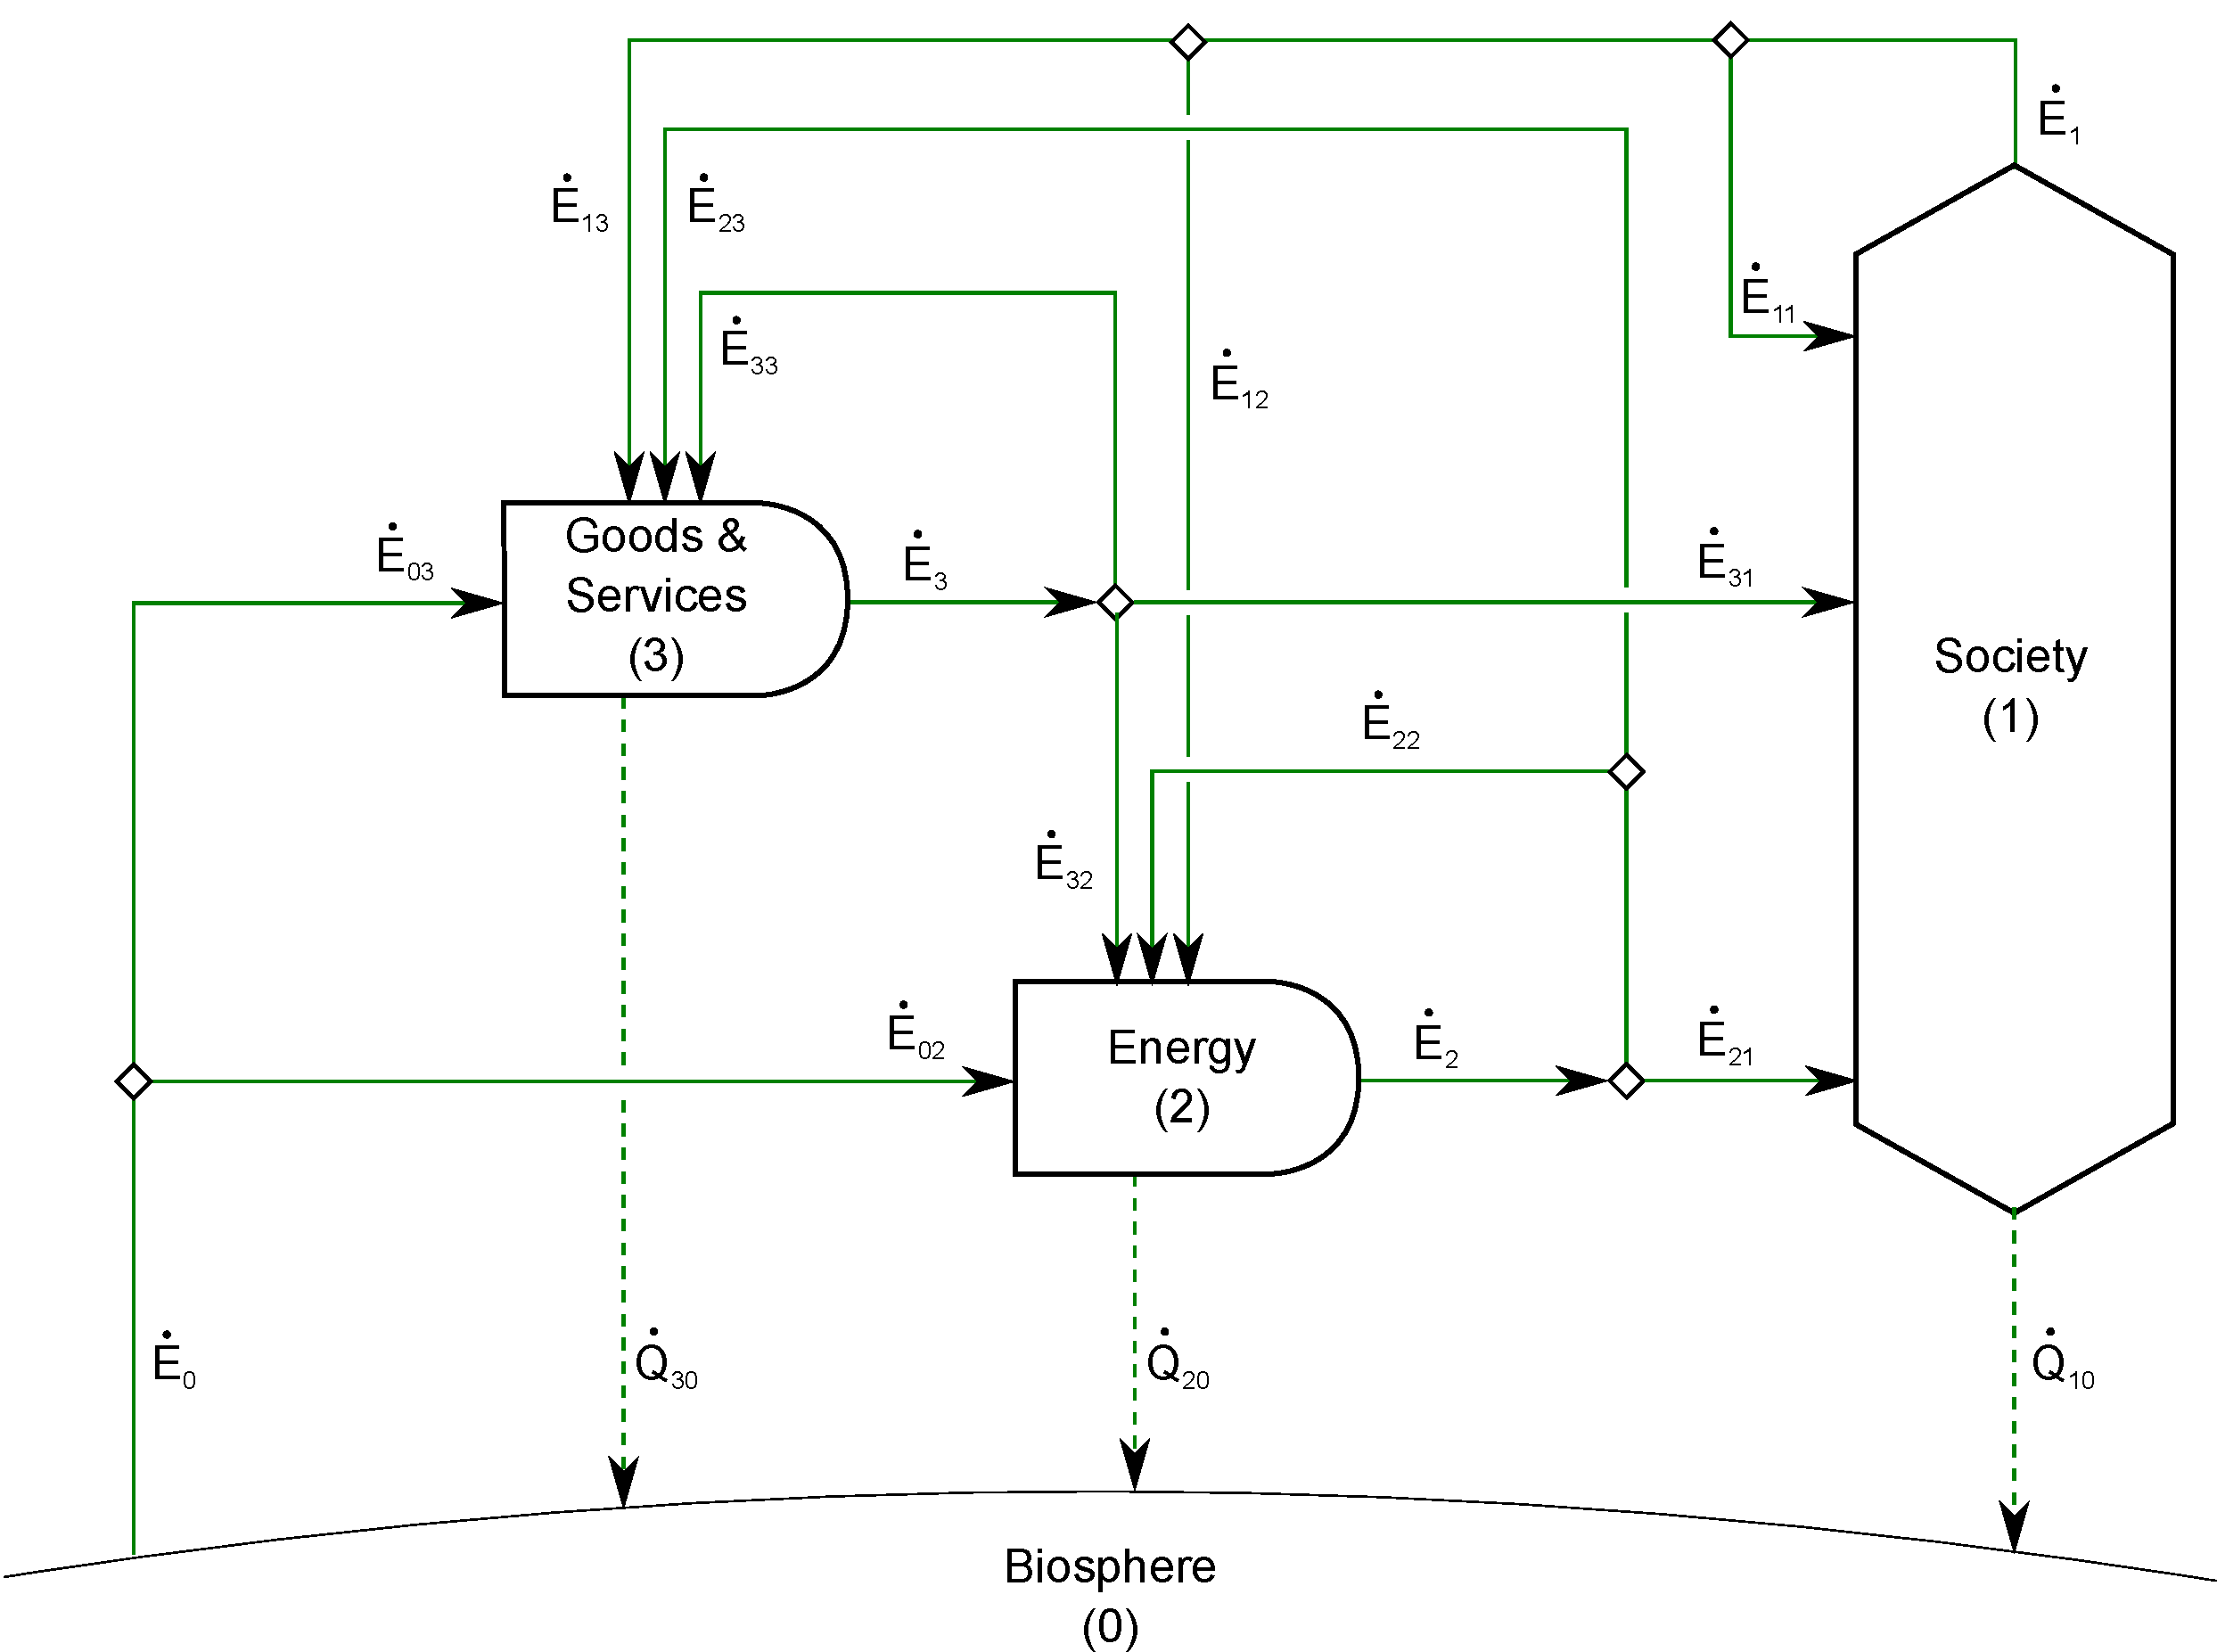
\includegraphics[width=0.8\linewidth]{Part_2/Chapter_Energy/images/3_sector_direct_energy.pdf}
\caption{Direct energy flows in Example C: a three-sector economy.}
\label{fig:C_energy}
\end{figure}

Both direct energy ($\dot{E}$) (such as chemical potential energy in coal, 
oil, and electricity) and waste heat ($\dot{Q}$) 
are accounted by the First Law of Thermodynamics. 
The First Law around the Goods and Services sector (4) including, 
for now, the accumulation rate of direct energy in the sector 
$\left(\frac{\mathrm{d}E_{4}}{\mathrm{d}t}\right)$ yields

\begin{equation} \label{eq:C-CV_E_dot_4}
	\frac{\mathrm{d}E_{4}}{\mathrm{d}t} 	 
	= \dot{E}_{14} 
	+ \dot{E}_{34} 
	+ \dot{E}_{44} 
	- \dot{E}_4 
	- \dot{Q}_{41}.
\end{equation}

Note that we may simplify Equation \ref{eq:C-CV_E_dot_4} 
by realizing that (a) $\dot{E}_{4} = \dot{E}_{4i} = 0$, 
because the goods and services sector 
is assumed to produce no flows of energy, 
and (b) $\dot{E}_{14} = 0$, 
because sector (4) receives no direct energy from the biosphere, 
except via the energy sector (3), hence:

\begin{equation} \label{eq:C-CV_E_dot_4_simp}
	\frac{\mathrm{d}E_{4}}{\mathrm{d}t} 	 
	= \dot{E}_{34} 
	- \dot{Q}_{41}.
\end{equation}

The First Law of Thermodynamics around the 
biosphere (1), society (2), and the energy sector (3) gives

\begin{equation} \label{eq:C-CV_E_dot_1}
	\frac{\mathrm{d}E_{1}}{\mathrm{d}t} 	 
	= \dot{Q}_{21} 
	+ \dot{Q}_{31} 
	+ \dot{Q}_{41} 
	- \dot{E}_{13} 
	- \dot{E}_{14},
\end{equation}

\begin{equation} \label{eq:C-CV_E_dot_2}
	\frac{\mathrm{d}E_{2}}{\mathrm{d}t}
	= \dot{E}_{32}  
	+ \dot{E}_{42} 
	- \dot{Q}_{21},
\end{equation}

\noindent and 

\begin{equation} \label{eq:C-CV_E_dot_3}
	\frac{\mathrm{d}E_{3}}{\mathrm{d}t} 	 
	= \dot{E}_{13} 
	+ \dot{E}_{33} 
	+ \dot{E}_{43} 
	- \dot{E}_{3} 
	- \dot{Q}_{31}.
\end{equation}

As in Examples A and B, we can set the accumulation of direct energy to zero.

\begin{equation} \label{eq:C-CV_E_dot_1_SS}
	0 
	= \dot{Q}_{21} 
	+ \dot{Q}_{31} 
	+ \dot{Q}_{41} 
	- \dot{E}_{13} 
	- \dot{E}_{14}
\end{equation}

\begin{equation} \label{eq:C-CV_E_dot_2_SS}
	0  
	= \dot{E}_{32} 
	+ \dot{E}_{42} 
	- \dot{Q}_{21}
\end{equation}

\begin{equation} \label{eq:C-CV_E_dot_3_SS}
	0 
	= \dot{E}_{13} 
	+ \dot{E}_{33} 
	+ \dot{E}_{43} 
	- \dot{E}_{3} 
	- \dot{Q}_{31}
\end{equation}

\noindent and 

\begin{equation} \label{eq:C-CV_E_dot_4_SS}
	0 
	= \dot{E}_{14} 
	+ \dot{E}_{34} 
	+ \dot{E}_{44} 
	- \dot{E}_4 
	- \dot{Q}_{41}
\end{equation}

In the next chapter, the above direct energy equations will be used to 
develop \emph{embodied} energy accounting equations for Examples A--C.




\bibliography{../../EROI_review_v2}
\bibliographystyle{unsrt}


% Always give a unique label
% and use \ref{<label>} for cross-references
% and \cite{<label>} for bibliographic references
% use \sectionmark{}
% to alter or adjust the section heading in the running head
%% Instead of simply listing headings of different levels we recommend to let every heading be followed by at least a short passage of text. Furtheron please use the \LaTeX\ automatism for all your cross-references and citations.

%% Please note that the first line of text that follows a heading is not indented, whereas the first lines of all sequent paragraphs are.

%% Use the standard \verb|equation| environment to typeset your equations, e.g.
%
%% \begin{equation}
%% a \times b = c\;,
%% \end{equation}
%
%% however, for multiline equations we recommend to use the \verb|eqnarray|
%% environment\footnote{In physics texts please activate the class option \texttt{vecphys} to depict your vectors in \textbf{\itshape boldface-italic} type - as is customary for a wide range of physical jects.}.
%% \begin{eqnarray}
%% a \times b = c \nonumber\\
%% \vec{a} \cdot \vec{b}=\vec{c}
%% \label{eq:01}
%% \end{eqnarray}

%% \section{section Heading}
%% \label{sec:2}
%% Instead of simply listing headings of different levels we recommend to let every heading be followed by at least a short passage of text. Furtheron please use the \LaTeX\ automatism for all your cross-references\index{cross-references} and citations\index{citations} as has already been described in Sect.~\ref{sec:2}.

%% \begin{quotation}
%% Please do not use quotation marks when quoting texts! Simply use the \verb|quotation| environment -- it will automatically render Springer's preferred layout.
%% \end{quotation}


%% \section{section Heading}
%% Instead of simply listing headings of different levels we recommend to let every heading be followed by at least a short passage of text. Furtheron please use the \LaTeX\ automatism for all your cross-references and citations as has already been described in Sect.~\ref{sec:2}, see also Fig.~\ref{fig:1}\footnote{If you copy text passages, figures, or tables from other works, you must obtain \textit{permission} from the copyright holder (usually the original publisher). Please enclose the signed permission with the manucript. The sources\index{permission to print} must be acknowledged either in the captions, as footnotes or in a separate section of the book.}

%% Please note that the first line of text that follows a heading is not indented, whereas the first lines of all sequent paragraphs are.

% For figures use
%
%% \begin{figure}[b]
%% \sidecaption
% Use the relevant command for your figure-insertion program
% to insert the figure file.
% For example, with the option graphics use
%% \includegraphics[scale=.65]{figure}
%
% If not, use
%\picplace{5cm}{2cm} % Give the correct figure height and width in cm
%
%% \caption{If the width of the figure is less than 7.8 cm use the \texttt{sidecapion} command to flush the caption on the left side of the page. If the figure is positioned at the top of the page, align the sidecaption with the top of the figure -- to achieve this you simply need to use the optional argument \texttt{[t]} with the \texttt{sidecaption} command}
%% \label{fig:1}       % Give a unique label
%% \end{figure}


%% \paragraph{Paragraph Heading} %
%% Instead of simply listing headings of different levels we recommend to let every heading be followed by at least a short passage of text. Furtheron please use the \LaTeX\ automatism for all your cross-references and citations as has already been described in Sect.~\ref{sec:2}.

%% Please note that the first line of text that follows a heading is not indented, whereas the first lines of all sequent paragraphs are.

%% For typesetting numbered lists we recommend to use the \verb|enumerate| environment -- it will automatically render Springer's preferred layout.

%% \begin{enumerate}
%% \item{Livelihood and survival mobility are oftentimes coutcomes of uneven socioeconomic development.}
%% \begin{enumerate}
%% \item{Livelihood and survival mobility are oftentimes coutcomes of uneven socioeconomic development.}
%% \item{Livelihood and survival mobility are oftentimes coutcomes of uneven socioeconomic development.}
%% \end{enumerate}
%% \item{Livelihood and survival mobility are oftentimes coutcomes of uneven socioeconomic development.}
%% \end{enumerate}


%% \paragraph{paragraph Heading} In order to avoid simply listing headings of different levels we recommend to let every heading be followed by at least a short passage of text. Use the \LaTeX\ automatism for all your cross-references and citations as has already been described in Sect.~\ref{sec:2}, see also Fig.~\ref{fig:2}.

%% Please note that the first line of text that follows a heading is not indented, whereas the first lines of all sequent paragraphs are.

%% For unnumbered list we recommend to use the \verb|itemize| environment -- it will automatically render Springer's preferred layout.

%% \begin{itemize}
%% \item{Livelihood and survival mobility are oftentimes coutcomes of uneven socioeconomic development, cf. Table~\ref{tab:1}.}
%% \begin{itemize}
%% \item{Livelihood and survival mobility are oftentimes coutcomes of uneven socioeconomic development.}
%% \item{Livelihood and survival mobility are oftentimes coutcomes of uneven socioeconomic development.}
%% \end{itemize}
%% \item{Livelihood and survival mobility are oftentimes coutcomes of uneven socioeconomic development.}
%% \end{itemize}

%% \begin{figure}[t]
%% \sidecaption[t]
% Use the relevant command for your figure-insertion program
% to insert the figure file.
% For example, with the option graphics use
%% \includegraphics[scale=.65]{figure}
%
% If not, use
%\picplace{5cm}{2cm} % Give the correct figure height and width in cm
%
%% \caption{Please write your figure caption here}
%% \label{fig:2}       % Give a unique label
%% \end{figure}

%% \runinhead{Run-in Heading Boldface Version} Use the \LaTeX\ automatism for all your cross-references and citations as has already been described in Sect.~\ref{sec:2}.

%% \runinhead{Run-in Heading Italic Version} Use the \LaTeX\ automatism for all your cross-refer\-ences and citations as has already been described in Sect.~\ref{sec:2}\index{paragraph}.
% Use the \index{} command to code your index words
%
% For tables use
%
%% \begin{table}
%% \caption{Please write your table caption here}
%% \label{tab:1}       % Give a unique label
%
% For LaTeX tables use
%
%% \begin{tabular}{p{2cm}p{2.4cm}p{2cm}p{4.9cm}}
%% \hline\noalign{\smallskip}
%% Classes & class & Length & Action Mechanism  \\
%% \noalign{\smallskip}\svhline\noalign{\smallskip}
%% Translation & mRNA$^a$  & 22 (19--25) & Translation repression, mRNA cleavage\\
%% Translation & mRNA cleavage & 21 & mRNA cleavage\\
%% Translation & mRNA  & 21--22 & mRNA cleavage\\
%%Translation & mRNA  & 24--26 & Histone and DNA Modification\\
%%\noalign{\smallskip}\hline\noalign{\smallskip}
%%\end{tabular}
%%$^a$ Table foot note (with superscript)
%%\end{table}
%
%% \section{Section Heading}
%%\label{sec:3}
% Always give a unique label
% and use \ref{<label>} for cross-references
% and \cite{<label>} for bibliographic references
% use \sectionmark{}
% to alter or adjust the section heading in the running head
%% Instead of simply listing headings of different levels we recommend to let every heading be followed by at least a short passage of text. Furtheron please use the \LaTeX\ automatism for all your cross-references and citations as has already been described in Sect.~\ref{sec:2}.

%% Please note that the first line of text that follows a heading is not indented, whereas the first lines of all sequent paragraphs are.

%%If you want to list definitions or the like we recommend to use the Springer-enhanced \verb|description| environment -- it will automatically render Springer's preferred layout.

%%\begin{description}[Type 1]
%%\item[Type 1]{That addresses central themes pertainng to migration, health, and disease. In Sect.~\ref{sec:1}, Wilson discusses the role of human migration in infectious disease distributions and patterns.}
%%\item[Type 2]{That addresses central themes pertainng to migration, health, and disease. In Sect.~\ref{sec:2}, Wilson discusses the role of human migration in infectious disease distributions and patterns.}
%%\end{description}

%%\section{section Heading} %
%% In order to avoid simply listing headings of different levels we recommend to let every heading be followed by at least a short passage of text. Use the \LaTeX\ automatism for all your cross-references and citations citations as has already been described in Sect.~\ref{sec:2}.

%% Please note that the first line of text that follows a heading is not indented, whereas the first lines of all sequent paragraphs are.

%% \begin{svgraybox}
%% If you want to emphasize complete paragraphs of texts we recommend to use the newly defined Springer class option \verb|graybox| and the newly defined environment \verb|svgraybox|. This will produce a 15 percent screened box 'behind' your text.

%% If you want to emphasize complete paragraphs of texts we recommend to use the newly defined Springer class option and environment \verb|svgraybox|. This will produce a 15 percent screened box 'behind' your text.
%% \end{svgraybox}


%% \section{section Heading}
%%Instead of simply listing headings of different levels we recommend to let every heading be followed by at least a short passage of text. Furtheron please use the \LaTeX\ automatism for all your cross-references and citations as has already been described in Sect.~\ref{sec:2}.

%% Please note that the first line of text that follows a heading is not indented, whereas the first lines of all sequent paragraphs are.

%% \begin{theorem}
%% Theorem text goes here.
%% \end{theorem}
%
% or
%
%% \begin{definition}
%% Definition text goes here.
%% \end{definition}

%% \begin{proof}
%\smartqed
%% Proof text goes here.
%% \qed
%% \end{proof}

%%\paragraph{Paragraph Heading} %
%% Instead of simply listing headings of different levels we recommend to let every heading be followed by at least a short passage of text. Furtheron please use the \LaTeX\ automatism for all your cross-references and citations as has already been described in Sect.~\ref{sec:2}.

%% Note that the first line of text that follows a heading is not indented, whereas the first lines of all subsequent paragraphs are.
%
% For built-in environments use
%
%%\begin{theorem}
%%Theorem text goes here.
%%\end{theorem}
%
%%\begin{definition}
%%Definition text goes here.
%%\end{definition}
%
%%\begin{proof}
%%\smartqed
%% Proof text goes here.
%%\qed
%%\end{proof}
%
%% \begin{acknowledgement}
%% If you want to include acknowledgments of assistance and the like at the end of an individual chapter please use the \verb|acknowledgement| environment -- it will automatically render Springer's preferred layout.
%% \end{acknowledgement}
%
%% \section*{Appendix}
%% \addcontentsline{toc}{section}{Appendix}
%
%% When placed at the end of a chapter or contribution (as opposed to at the end of the book), the numbering of tables, figures, and equations in the appendix section continues on from that in the main text. Hence please \textit{do not} use the \verb|appendix| command when writing an appendix at the end of your chapter or contribution. If there is only one the appendix is designated ``Appendix'', or ``Appendix 1'', or ``Appendix 2'', etc. if there is more than one.

%% \begin{equation}
%% a \times b = c
%% \end{equation}
% Problems or Exercises should be sorted chapterwise
%% \section*{Problems}
%% \addcontentsline{toc}{section}{Problems}
%
% Use the following environment.
% Don't forget to label each problem;
% the label is needed for the solutions' environment
%% \begin{prob}
%% \label{prob1}
%% A given problem or Excercise is described here. The
%% problem is described here. The problem is described here.
%% \end{prob}

%% \begin{prob}
%% \label{prob2}
%% \textbf{Problem Heading}\\
%% (a) The first part of the problem is described here.\\
%% (b) The second part of the problem is described here.
%% \end{prob}


